% Options for packages loaded elsewhere
\PassOptionsToPackage{unicode}{hyperref}
\PassOptionsToPackage{hyphens}{url}
\documentclass[
]{article}
\usepackage{xcolor}
\usepackage{amsmath,amssymb}
\setcounter{secnumdepth}{5}
\usepackage{iftex}
\ifPDFTeX
  \usepackage[T1]{fontenc}
  \usepackage[utf8]{inputenc}
  \usepackage{textcomp} % provide euro and other symbols
\else % if luatex or xetex
  \usepackage{unicode-math} % this also loads fontspec
  \defaultfontfeatures{Scale=MatchLowercase}
  \defaultfontfeatures[\rmfamily]{Ligatures=TeX,Scale=1}
\fi
\usepackage{lmodern}
\ifPDFTeX\else
  % xetex/luatex font selection
\fi
% Use upquote if available, for straight quotes in verbatim environments
\IfFileExists{upquote.sty}{\usepackage{upquote}}{}
\IfFileExists{microtype.sty}{% use microtype if available
  \usepackage[]{microtype}
  \UseMicrotypeSet[protrusion]{basicmath} % disable protrusion for tt fonts
}{}
\makeatletter
\@ifundefined{KOMAClassName}{% if non-KOMA class
  \IfFileExists{parskip.sty}{%
    \usepackage{parskip}
  }{% else
    \setlength{\parindent}{0pt}
    \setlength{\parskip}{6pt plus 2pt minus 1pt}}
}{% if KOMA class
  \KOMAoptions{parskip=half}}
\makeatother
\usepackage{longtable,booktabs,array}
\usepackage{calc} % for calculating minipage widths
% Correct order of tables after \paragraph or \subparagraph
\usepackage{etoolbox}
\makeatletter
\patchcmd\longtable{\par}{\if@noskipsec\mbox{}\fi\par}{}{}
\makeatother
% Allow footnotes in longtable head/foot
\IfFileExists{footnotehyper.sty}{\usepackage{footnotehyper}}{\usepackage{footnote}}
\makesavenoteenv{longtable}
\usepackage{graphicx}
\makeatletter
\newsavebox\pandoc@box
\newcommand*\pandocbounded[1]{% scales image to fit in text height/width
  \sbox\pandoc@box{#1}%
  \Gscale@div\@tempa{\textheight}{\dimexpr\ht\pandoc@box+\dp\pandoc@box\relax}%
  \Gscale@div\@tempb{\linewidth}{\wd\pandoc@box}%
  \ifdim\@tempb\p@<\@tempa\p@\let\@tempa\@tempb\fi% select the smaller of both
  \ifdim\@tempa\p@<\p@\scalebox{\@tempa}{\usebox\pandoc@box}%
  \else\usebox{\pandoc@box}%
  \fi%
}
% Set default figure placement to htbp
\def\fps@figure{htbp}
\makeatother
\setlength{\emergencystretch}{3em} % prevent overfull lines
\providecommand{\tightlist}{%
  \setlength{\itemsep}{0pt}\setlength{\parskip}{0pt}}
\usepackage[]{natbib}
\bibliographystyle{plainnat}
\usepackage{fontspec}
\setmainfont{STIX Two Text}
\setsansfont{STIX Two Text}
\setmonofont{Menlo}
\usepackage{float}
\floatplacement{figure}{H}
\usepackage[margin=1in]{geometry}
\usepackage{microtype}
\usepackage{booktabs}
\usepackage{longtable}
\usepackage{array}
\usepackage{calc}
\usepackage{etoolbox}
\usepackage{xcolor}
\usepackage{url}
\AtBeginDocument{%
  \let\oldurl\url
  \renewcommand{\url}[1]{\mbox{\oldurl{#1}}}%
}
\renewcommand{\bibfont}{\small}
\usepackage{titlesec}
\AtBeginEnvironment{longtable}{\footnotesize}
\AtBeginEnvironment{thebibliography}{\raggedright}
\setlength{\LTcapwidth}{\linewidth}
\setlength{\parskip}{0pt}
\setlength{\parindent}{1.2em}
\titlespacing*{\section}{0pt}{1.2ex plus 0.2ex}{0.45ex}
\titlespacing*{\subsection}{0pt}{1.0ex plus 0.2ex}{0.35ex}
\setlength{\abovedisplayskip}{4pt}
\setlength{\belowdisplayskip}{4pt}
\usepackage{bookmark}
\IfFileExists{xurl.sty}{\usepackage{xurl}}{} % add URL line breaks if available
\urlstyle{same}
\hypersetup{
  pdftitle={Sampling more only helps if you can select},
  pdfauthor={Kaivalya Singh},
  hidelinks,
  pdfcreator={LaTeX via pandoc}}

\title{Sampling more only helps if you can select}
\usepackage{etoolbox}
\makeatletter
\providecommand{\subtitle}[1]{% add subtitle to \maketitle
  \apptocmd{\@title}{\par {\large #1 \par}}{}{}
}
\makeatother
\subtitle{A within-issue audit of label-free selection signals for
software-engineering agents}
\author{Kaivalya Singh}
\date{1 November 2026}

\begin{document}
\maketitle
\begin{abstract}
Software-engineering agents can sample several patches per issue, but
deployment must submit one without evaluation labels. We audit selection
on 94,341 issue-by-configuration units over 41,073 issues (48,300 before
filtering) from two public trajectory corpora: eleven three-attempt
configurations and one eight-attempt arm. Resolve outcomes are largely a
property of the issue (ICC 0.646--0.864), and the fixed-budget curve
f(k) moves by at most 1.07 percentage points. Oracle pass@K exceeds the
selected rate by 4.82--15.75 points, but cheap signals remain weak
(AUROC 0.51--0.58) and do not close the gap. Agreement is nominally
above a random draw in 7 of 11 configurations (sign test p = 0.549); own
tests give a within-issue AUROC of 0.5125 (95\% CI 0.4973--0.5286, p =
0.119). Cross-fit difficulty certifies 2/11, 10/11, and 11/11 K=3
configurations at α = 0.05, 0.10, 0.20, versus 0/11, 0/11, and 2/11 for
agreement, but needs sibling labels and was not blind. A local Gemma 4
26B-A4B Q4\_0 judge reaches 0.5786 (0.5587--0.5987), a small uncorrected
edge over exit reason (+0.0209, 95\% CI +0.0025 to +0.0411); it
misorders about 42\% of mixed pairs. Sampling more alone does not make
selection deployable with the label-free signals these trajectories
contain.
\end{abstract}

\section{Introduction}\label{introduction}

Software-engineering agents edit repositories, run tests, and iterate
\citep{yang2024sweagent, wang2024openhands}. Drawing K trajectories per
issue spends more inference compute
\citep{brown2024monkeys, snell2024scaling}. Coverage rises; the
submitted patch's resolve rate does not. That gap is selection, which
deployment must solve without labels.

We audit selection on frozen trajectories with K attempts per issue. How
much variance is between issues, and how flat is f(k)? Within an issue,
can cheap signals rank a resolved attempt above an unresolved one? Does
a local judge add information?

We contribute between-issue structure on 94,341 units over 41,073 issues
from 48,300 across twelve arms (ICC, f(k), selection gap); a kill test
with label-convention and no-coverage reporting; four pre-registered
tests (B1 agreement lift, B2 own-test ranking, B3 cross-fit
certification, B4 repeated-patch stopping) and one exploratory test (B5
own-test stopping); and a Gemma 4 judge on 4,226 pairs.

\section{Related work}\label{related-work}

SWE-bench defined repository-level issue resolution
\citep{jimenez2023swebench}; SWE-agent, OpenHands and Agentless made the
execution loop and repair pipelines central
\citep{yang2024sweagent, wang2024openhands, xia2024agentless}. Corpora:
Nebius OpenHands \citep{nebius2025trajectories} and NVIDIA
Open-SWE-Traces \citep{nvidia2026traces, ahmad2026openswe}.

Repeated sampling and selective prediction are the closest work
\citep{wang2022selfconsistency, brown2024monkeys, geifman2017selective};
Learn-then-Test supplies the kill test \citep{angelopoulos2021ltt} and
LLM judges are scalable \citep{zheng2023judge}.

\section{Setup}\label{setup}

\subsection{Data and frozen frames}\label{data-and-frozen-frames}

Nebius supplies 67,074 OpenHands trajectories over 6,306 issues and
1,823 repositories \citep{nebius2025trajectories}. NVIDIA supplies
818,660 rows in 32 configurations over 42,545 casefolded issues and
3,787 repositories \citep{nvidia2026traces}. We exclude 204 shared
issues. The post-overlap, pre-floor sets are \textbf{pools}: Nebius
6,102; NVIDIA 42,198. NVIDIA's 42,341 is 42,402 frozen-config issues
minus 204 shared, plus 143 non-frozen-only. Labels are the published
\texttt{resolved} flags; neither harness was rerun.

The frozen analysis has eleven K=3 configurations and one Nebius K=8
arm: 94,341 units over 41,073 issues clearing the three-attempt floor
(6,063 Nebius and 35,010 NVIDIA; 39 and 7,188 below K=3). The K=3 set is
Nebius, four v1.0, four v1.1, and two v1.2 slices (Table 3). K=8 reuses
Nebius K=3's 4,580 issues, adding none distinct. Six of eleven K=3 arms
use 27B language models (four Qwen3.6, two Qwen3.8; 28B total with
vision), comparable in size to Gemma 4 26B-A4B and 31B; we do not claim
local execution.

\begin{figure}
\centering
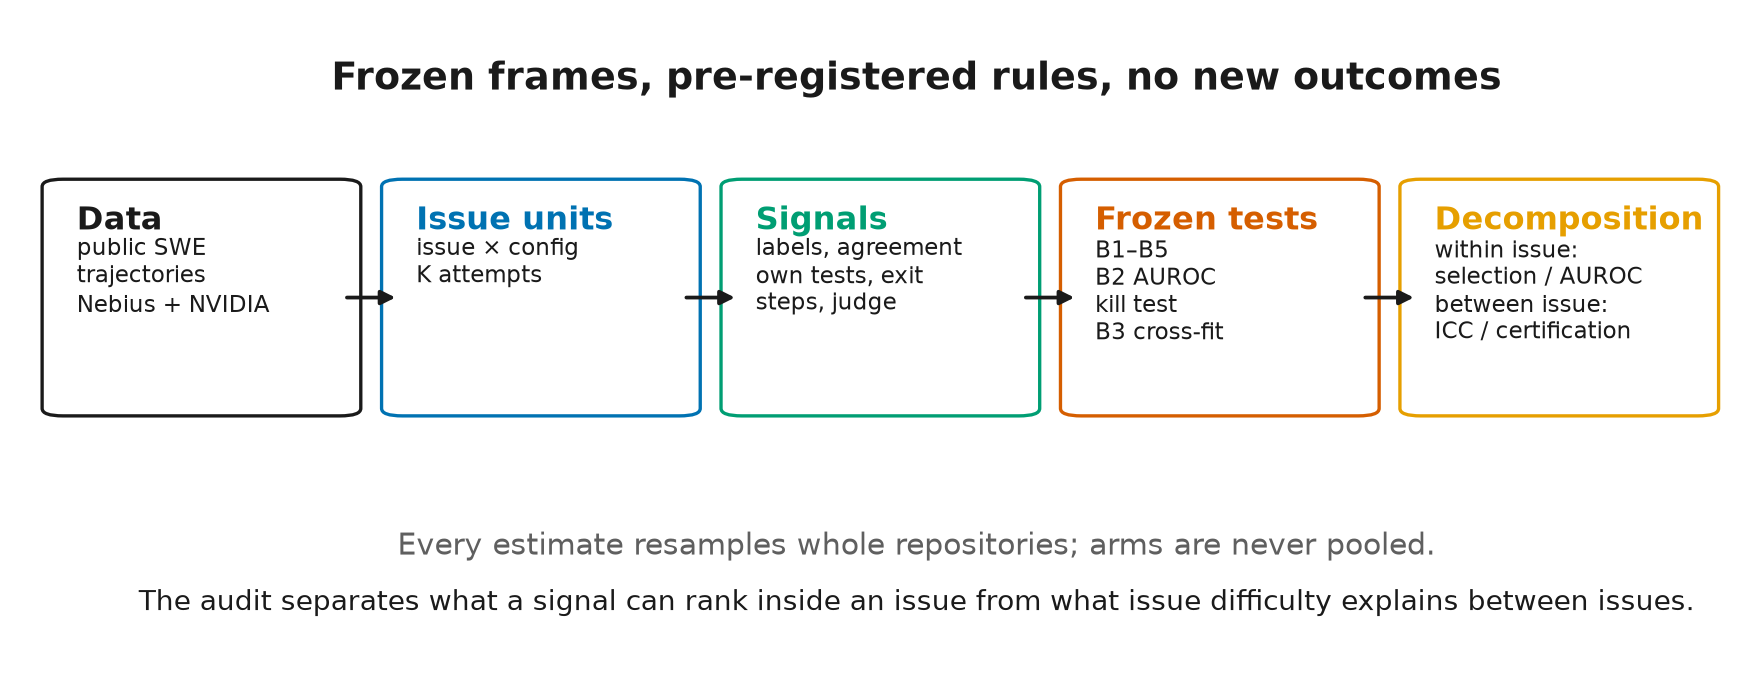
\includegraphics[width=1\linewidth,height=\textheight,keepaspectratio,alt={Design. Public trajectories to issue-by-configuration units with K attempts, five signals, frozen tests, and within- versus between-issue analyses. No new outcomes. Source: frozen pre-registration and DEVIATIONS.md.}]{figures/fig1_design.png}
\caption{Design. Public trajectories to issue-by-configuration units
with K attempts, five signals, frozen tests, and within- versus
between-issue analyses. No new outcomes. Source: frozen pre-registration
and DEVIATIONS.md.}\label{fig:design}
\end{figure}

\subsection{Units, rule, and signals}\label{units-rule-and-signals}

Each configuration-issue unit has K attempts. The submission represents
the largest canonical cluster. When several clusters tie for largest, B1
chooses one by a seeded random draw over the tied clusters (as frozen in
PREREG-2) and then takes that cluster's smallest
\texttt{trajectory\_id}; B4 breaks ties by the smallest
\texttt{trajectory\_id}; the kill test/\texttt{rate\_loo} take the
lexicographically smallest canonical cluster. Its label is the outcome.
Oracle pass@K is one if any attempt resolved; \texttt{f(k)} is the
plurality-cluster rate using the first k seeded draws; the gap is oracle
minus selected.

Strict canonicalisation (scratch files, reordered hunks, equivalent
edits) makes agreement conservative. The primary convention drops
\texttt{resolved\ =\ −1}; scoring it as failure changes pool and labels.
On NVIDIA, \texttt{−1} is 9.48\% of SWE-rebench-V2 rows and 4.85\% of
Scale-SWE rows.

Five signals. Agreement is the largest canonical cluster's share. Own
tests is \texttt{pred\_passes\_gen\_tests}, null when unavailable. Exit
reason is \texttt{submit} versus max-iteration. Steps is the
assistant-message count; the pre-registered score is raw, and resolved
attempts tend to use fewer messages (raw AUROC 0.4397; oriented 0.5603,
post-hoc). Cross-fit difficulty is
\texttt{rate\_loo\ =\ (Σ\ resolved\ −\ resolved\_rep)/(K−1)}, the
resolve rate of the other K−1 attempts; it needs those attempts
evaluated first.

The judge reads the issue and one patch and returns a single-token
YES/NO judgment; \texttt{p\_yes} is a two-way softmax over the YES/NO
logits. Issue text is truncated to 3,072 head and 1,024 tail tokens;
patches to 4,096 and 1,024.

\subsection{Inference and
pre-registration}\label{inference-and-pre-registration}

Intervals are 95\% percentile bootstraps over whole repositories (B =
2,000), because attempts within an issue are dependent. B1 and B4 use
Holm over the eleven K=3 configurations plus an exact sign test. B2 is a
single test: SIGNIFICANT+ requires two-sided p \textless{} 0.05 and a CI
excluding 0.5. B3 uses an exact sign test. K=8 is always separate and
enters no family.

B5 is exploratory. Deviations are named descriptively in DEVIATIONS.md.

The kill test is fixed-sequence Learn-then-Test over a pre-registered τ
grid, δ = 0.05, at least 30 calibration issues, on random-issue,
held-out-repo, and temporal splits at α = 0.05, 0.10, 0.20. B1--B4 were
frozen at \texttt{f9558d9} in PREREG-2. The post-freeze amendments are
D9.1 (B2's frozen K=8 draw is 4,226 pairs over 754 issues, not 11,611
over 943), D9.2 (the kill test's cluster tie-break) and D9.3 (the
sign-test threshold is 10--1); none changed a reported frozen result,
but D9.2 means the kill test and B3 used a tie-break other than the
frozen text (smallest \texttt{trajectory\_id}), moving full-budget
resolve by −1.83 to +1.08 pp.~Descriptive tables compute no test. The
judge study was frozen in its own pre-registration, under the documented
Q4\_0 substitution (DEVIATIONS.md), before any score existed.

\section{Results}\label{results}

\subsection{Issue difficulty dominates, and f(k) is
flat}\label{issue-difficulty-dominates-and-fk-is-flat}

Coverage rises with K, but the selected rate does not. Pass@1 is
32.29--59.49\%, plurality-cluster selected 32.20--59.44\% (largest
canonical cluster, ties by smallest \texttt{trajectory\_id}), and oracle
pass@K 41.70--64.30\% (Figure 2). The selection gap is 4.82--15.75
points across K=3 and 11.24 for K=8. Point estimates only. When patches
rarely coincide, the plurality-cluster rule reduces to a near-random
pick, so flat f(k) restates B1's null; the informative quantity is the
gap to oracle.

\begin{figure}
\centering
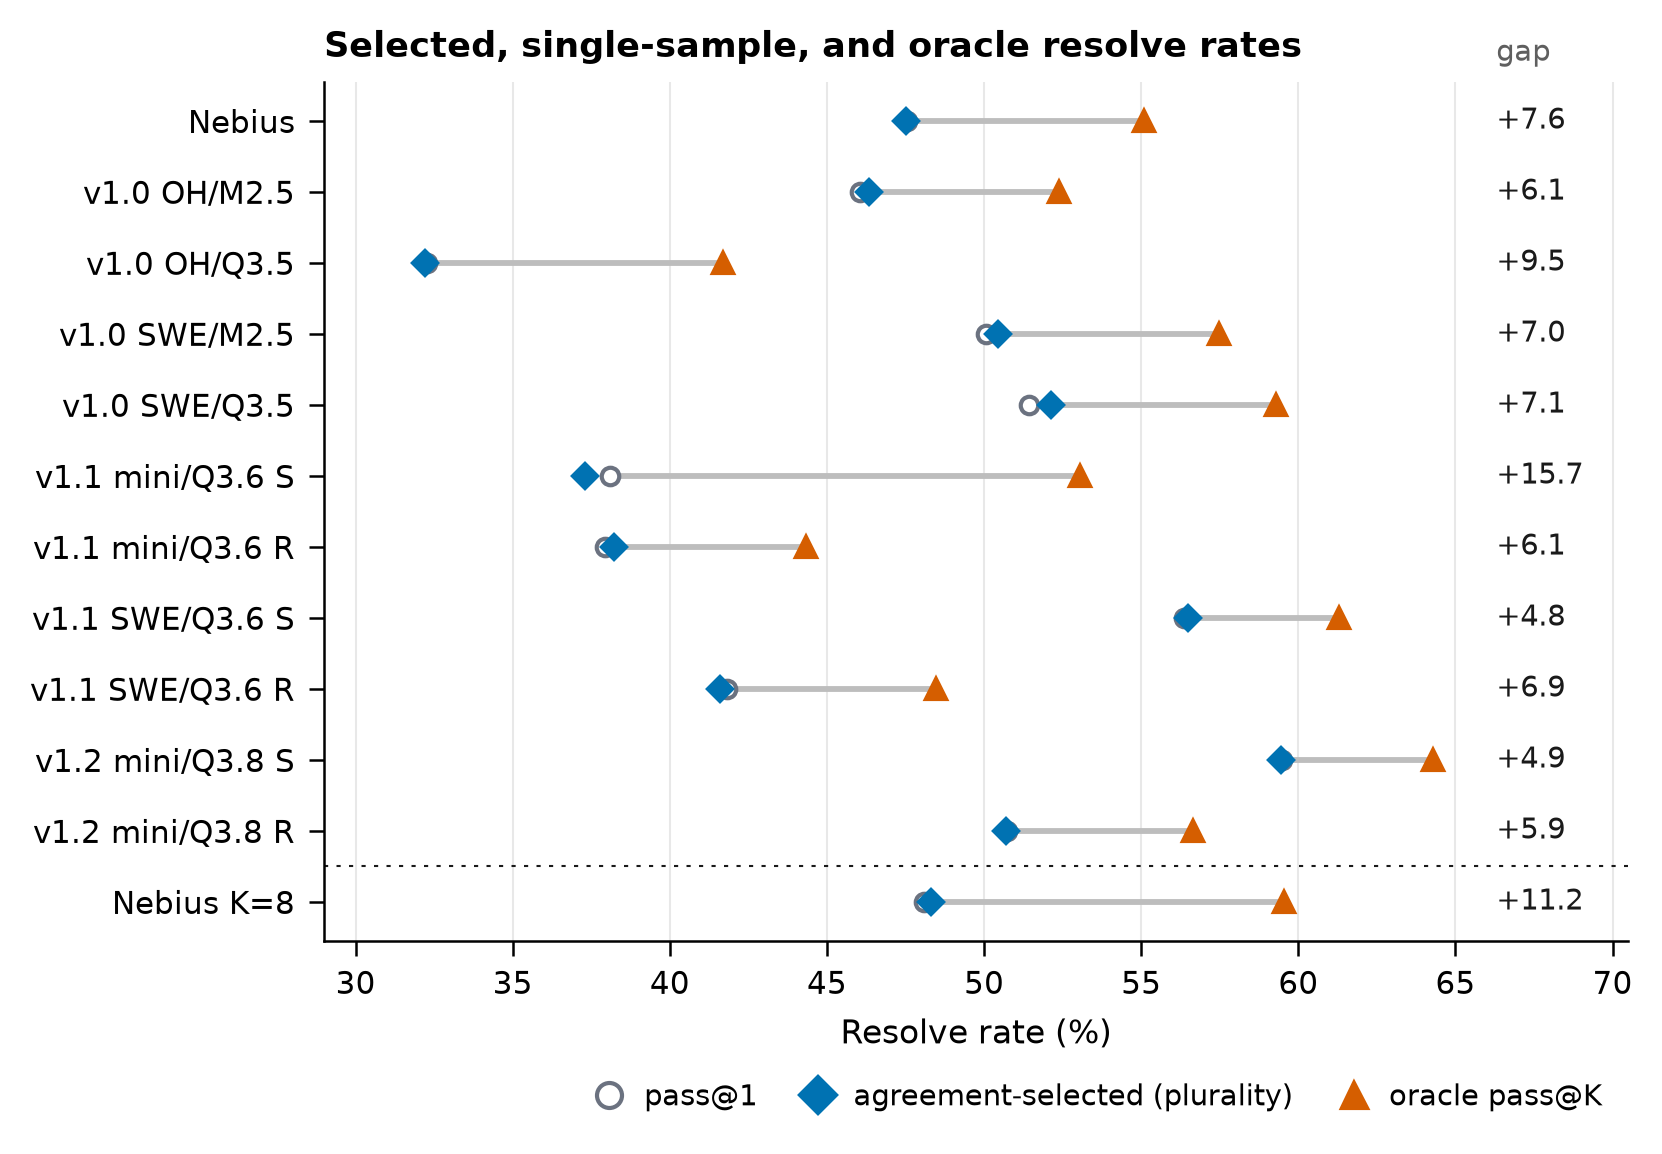
\includegraphics[width=0.95\linewidth,height=\textheight,keepaspectratio,alt={Per arm: pass@1 (circle), plurality-cluster selected (diamond), oracle pass@K (triangle); line = gap. Selected: largest canonical cluster, ties by smallest trajectory\_id. 12 arms, 94,341 units over 41,073 issues; point estimates. Source: results/descriptive\_tables.json, results/paper\_addenda.json.}]{figures/fig2_selection_gap.png}
\caption{Per arm: pass@1 (circle), plurality-cluster selected (diamond),
oracle pass@K (triangle); line = gap. Selected: largest canonical
cluster, ties by smallest \texttt{trajectory\_id}. 12 arms, 94,341 units
over 41,073 issues; point estimates. Source:
\texttt{results/descriptive\_tables.json},
\texttt{results/paper\_addenda.json}.}\label{fig:gap}
\end{figure}

f(k) is flat: across all twelve arms it moves at most 1.07 points (0.68
for K=8; Figure 3).

\begin{figure}
\centering
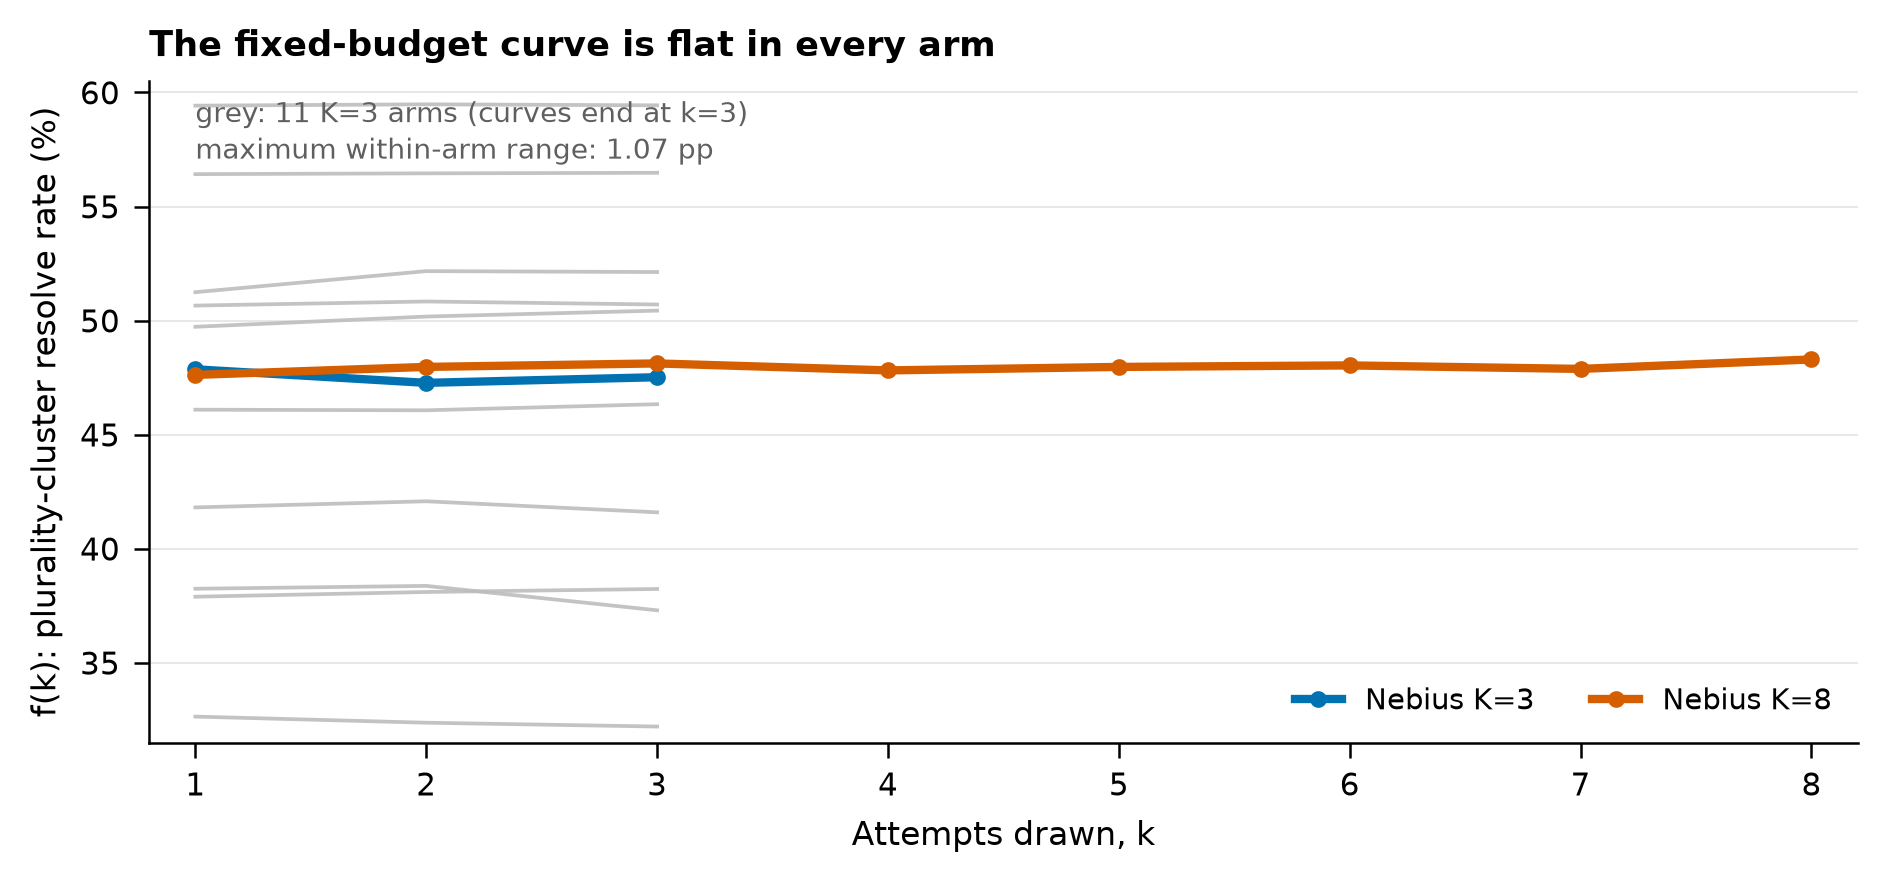
\includegraphics[width=0.95\linewidth,height=\textheight,keepaspectratio,alt={f(k), plurality-cluster resolve rate at budget k, every arm; K=3 ends at 3. Maximum range 1.07 pp; point estimates. Source: results/descriptive\_tables.json.}]{figures/fig3_fixed_budget.png}
\caption{f(k), plurality-cluster resolve rate at budget k, every arm;
K=3 ends at 3. Maximum range 1.07 pp; point estimates. Source:
\texttt{results/descriptive\_tables.json}.}\label{fig:curves}
\end{figure}

ICC is 0.646--0.864 across twelve arms (Figure 4); Nebius K=8 is 0.798
(95\% CI 0.787--0.811), K=3 0.795 (0.782--0.807). Most label variance is
between issues; only 14--35\% remains to distinguish attempts, which is
why the within-issue tests are noisy.

\begin{figure}
\centering
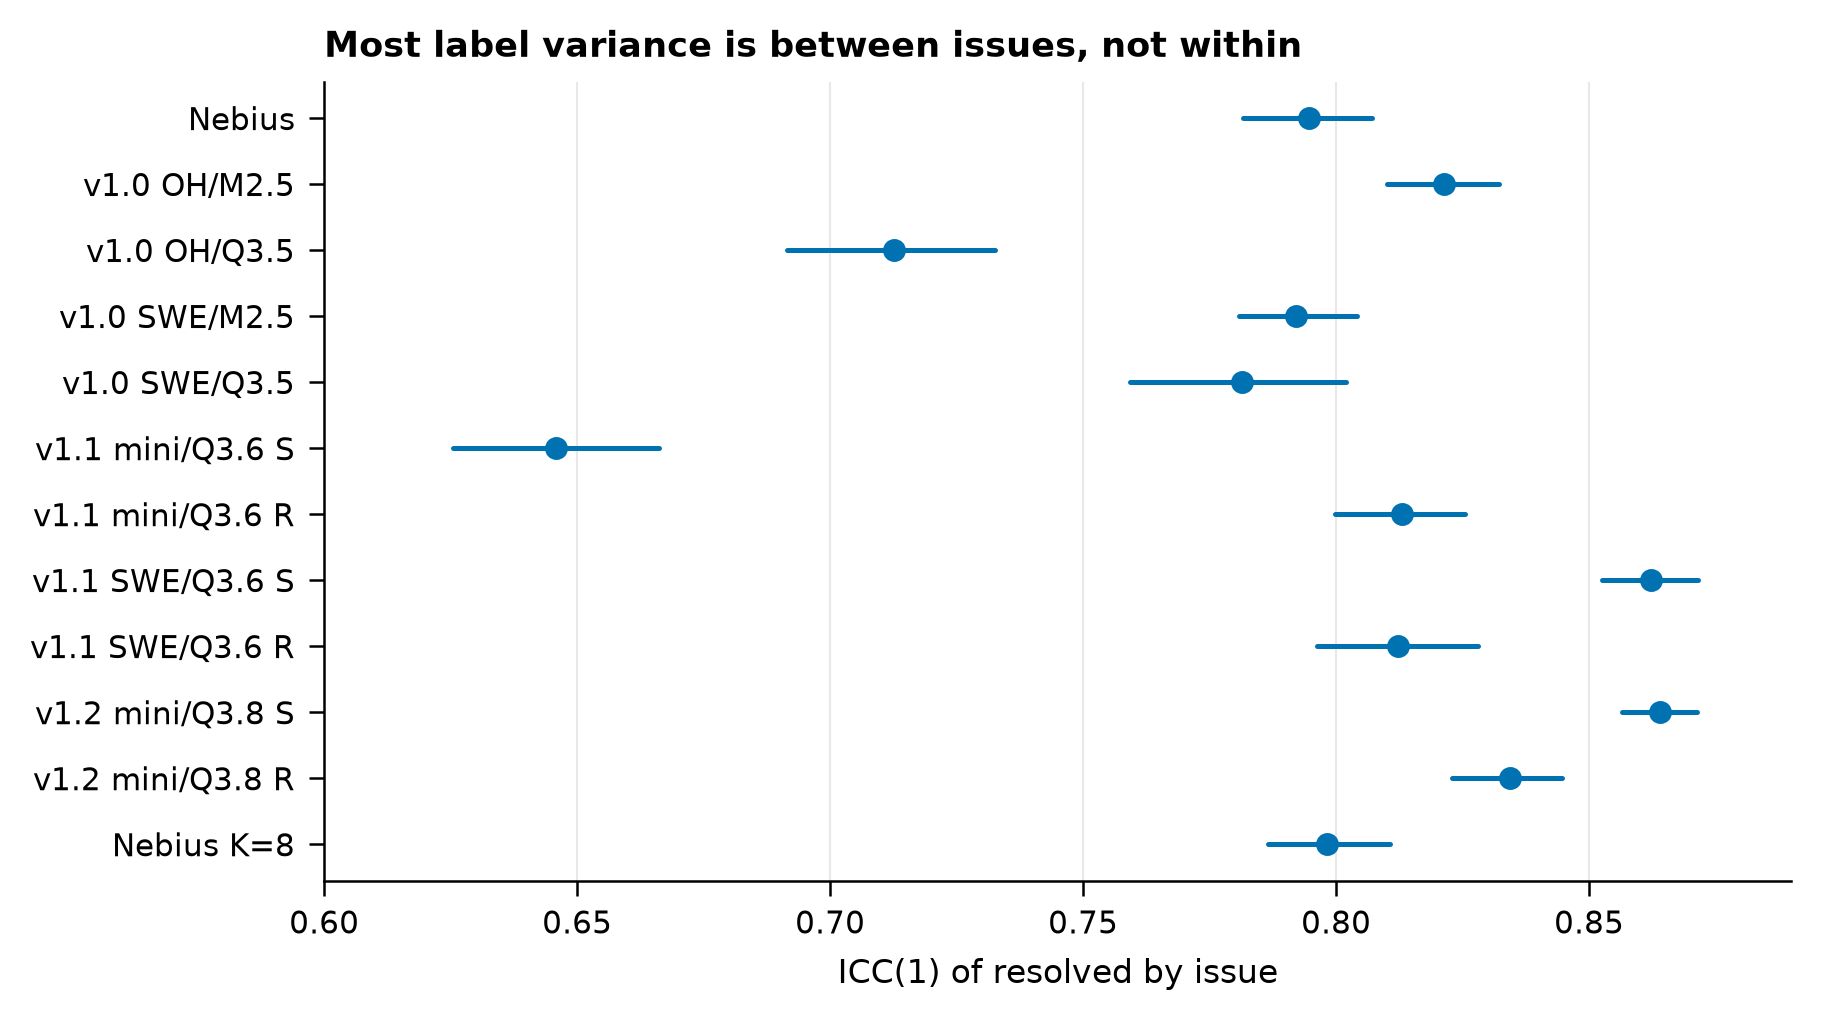
\includegraphics[width=0.95\linewidth,height=\textheight,keepaspectratio,alt={ICC(1) of resolved by issue, 12 arms, 95\% repo-clustered bootstrap (B = 2,000); range 0.646--0.864, K=8 0.798. Source: results/descriptive\_tables.json.}]{figures/fig4_icc.png}
\caption{ICC(1) of \texttt{resolved} by issue, 12 arms, 95\%
repo-clustered bootstrap (B = 2,000); range 0.646--0.864, K=8 0.798.
Source: \texttt{results/descriptive\_tables.json}.}\label{fig:icc}
\end{figure}

\subsection{Kill test: 0 BREAKS, two arms, and label
sensitivity}\label{kill-test-0-breaks-two-arms-and-label-sensitivity}

The agreement rule produced \textbf{0 BREAKS across 189 distinct cells}.
A cell is configuration × split × α × label convention. There are 99 per
convention: 90 K=3 (eight configurations on three splits; three
Scale-SWE on two, lacking \texttt{created\_at}) plus nine K=8; the K=8
cells are identical across conventions, so 90×2 + 9 = 189. Certification
was 0/12, 0/12, 2/12 at α = 0.05, 0.10, 0.20. Ten arms are NO-COVERAGE
at every α (no threshold met the risk target), not a pass. Certified
cells: coverage 7.14\% and 5.58\%; held-out risk 15.8\% (11.7--20.1\%)
and 16.4\% (12.4--20.6\%).

The label convention decides the verdict. Scoring \texttt{−1} as failure
raises risk to 24.0\% and 27.1\%, above 0.20; the pipeline certifies
0/12 arms at every α. We call neither primary. Secondary files-touched
agreement is 0/11 K=3 configurations at every α; patch size and steps
0/11 at 0.20.

Cross-fit: 2/11, 10/11, 11/11 K=3 configurations vs 0/11, 0/11, 2/11 for
agreement (Figure 6); K=8 certifies at all three, agreement at none. At
0.20 coverage is 27.1--63.9\% and risk 4.4--15.2\%. It is neither free
nor blind: deploying it requires evaluating the other K−1 attempts.

\subsection{B1 and B2: agreement is tiny, own tests are
weak}\label{b1-and-b2-agreement-is-tiny-own-tests-are-weak}

B1's lift is selected minus random-K, where random-K is the issue's own
rate. On non-mixed issues both terms are the same label, so lift is zero
by construction; the mean comes only from mixed issues. The family is
7+/4− (p = 0.549), with one negative Holm survivor: v1.1 mini/Qwen3.6
Scale-SWE, −0.755 pp {[}−1.207, −0.319{]}, Holm 0.022.

B2's Nebius K=8 own-test AUROC is 0.5125 (95\% CI 0.4973--0.5286, p =
0.119) on 4,226 pairs over 754 issues and 443 repositories; the CI
includes 0.5, so the rule returns NOT SIGNIFICANT. Agreement is 0.5058
(0.5018--0.5112, p = 0.0020), tiny but detectable; exit reason 0.5764
(0.5578--0.5939); steps 0.4397 (0.4146--0.4649), meaning resolved
attempts use fewer messages. The post-hoc oriented score is 0.5603
(0.5351--0.5854), a weak signal (\textbar AUROC − 0.5\textbar{} =
0.060).

The own-test selection lift is +0.892 pp (0.268--1.519, p = 0.005),
report-only; E2 null-zero is +0.871 (0.203--1.527). E1's own-test
AUROCs, on pairs where both attempts have non-null own-test results, are
0.5063 (both submitted) and 0.5066 (both max-iteration), so
within-stratum discrimination is absent; the pooled 0.5125 may come from
exit-reason-differing pairs. E1's stratified lifts are exploratory and
uncorrected across strata: +0.67 pp (0.03--1.32) where all eight
submitted (3,299 issues), +1.39 (−0.07--2.93) where exits are mixed
(1,239), and +3.27 (−5.21--11.61) on 42 all-max issues. When every
attempt has a test result (226 issues), the lift is −0.22 pp (95\% CI
−4.04 to +3.76, p = 0.977). The minimum detectable effect is about 5.6
pp at 80\% power, roughly six times the pooled +0.892 pp, so this subset
cannot test whether the pooled lift reflects test availability.

\begin{figure}
\centering
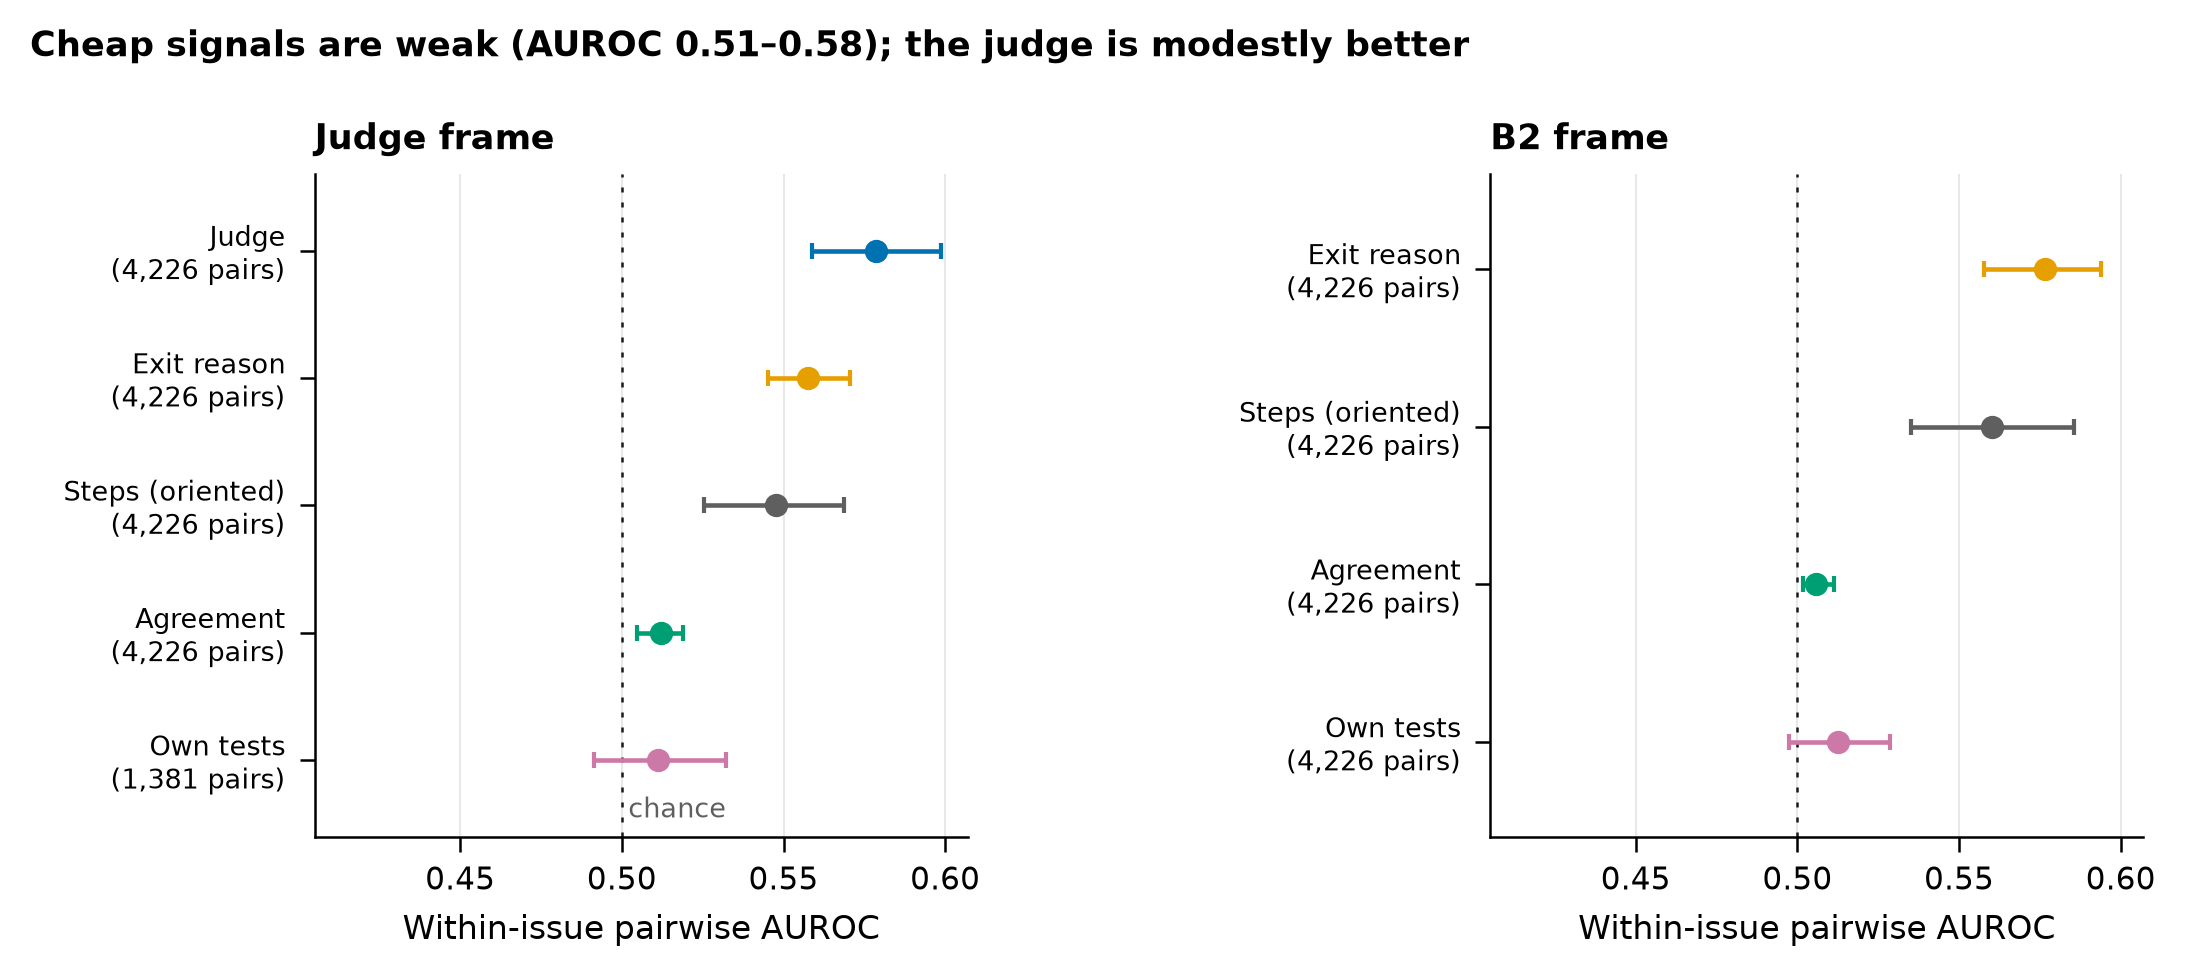
\includegraphics[width=1\linewidth,height=\textheight,keepaspectratio,alt={Mixed-label within-issue pairwise AUROC, 95\% repo-clustered bootstrap (B = 2,000). Left: judge frame (4,226 pairs; own tests 1,381); right: B2 frame, Nebius K=8 only (4,226). Steps oriented (0.5603; raw 0.4397). Sources: judge\_analysis.json, b2\_within\_issue\_auroc.json.}]{figures/fig5_auroc.png}
\caption{Mixed-label within-issue pairwise AUROC, 95\% repo-clustered
bootstrap (B = 2,000). Left: judge frame (4,226 pairs; own tests 1,381);
right: B2 frame, Nebius K=8 only (4,226). Steps oriented (0.5603; raw
0.4397). Sources: \texttt{judge\_analysis.json},
\texttt{b2\_within\_issue\_auroc.json}.}\label{fig:auroc}
\end{figure}

\subsection{B3: certifies, but not free and not
blind}\label{b3-certifies-but-not-free-and-not-blind}

B3 compares cross-fit and agreement identically: 11--0, p \textless=
0.001; \texttt{−1}-as-failure also 11--0; K=8 3 vs 0. \texttt{rate\_loo}
needs the other K−1 labels and uses the kill test's canonical-string
tie-break (DEVIATIONS.md); its headline existed before PREREG-2. It is
evidence that difficulty is measurable from sibling labels, not for a
free selector.

\begin{figure}
\centering
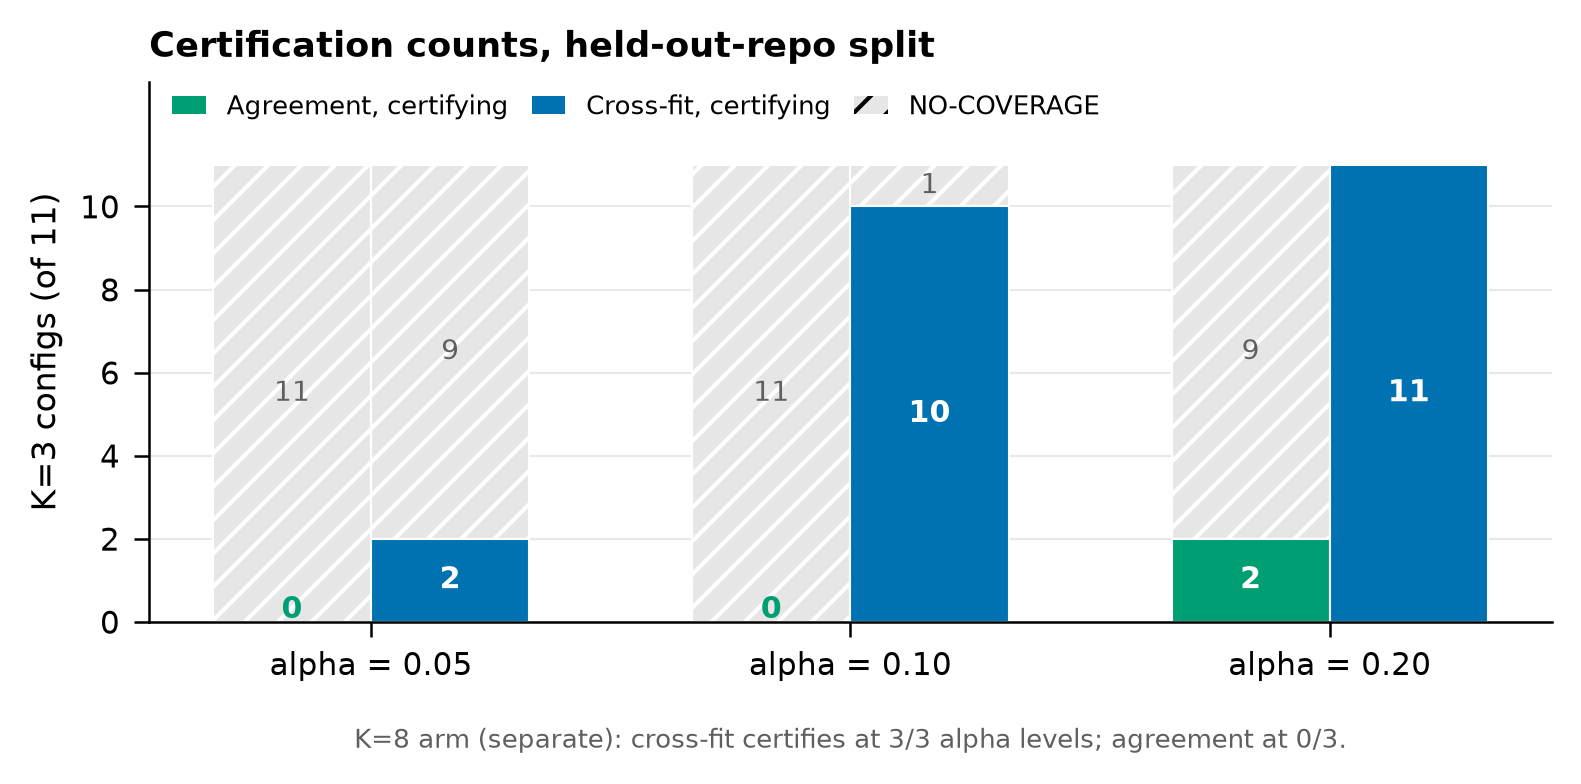
\includegraphics[width=0.85\linewidth,height=\textheight,keepaspectratio,alt={Held-out-repo certification, 11 K=3 configurations, α = 0.05/0.10/0.20; solid = certify, hatched = NO-COVERAGE. Agreement 0/0/2; cross-fit 2/10/11; K=8 cross-fit 3/3, agreement 0/3. Sources: b3\_crossfit\_certification.json, kill\_test.json.}]{figures/fig6_certification.png}
\caption{Held-out-repo certification, 11 K=3 configurations, α =
0.05/0.10/0.20; solid = certify, hatched = NO-COVERAGE. Agreement 0/0/2;
cross-fit 2/10/11; K=8 cross-fit 3/3, agreement 0/3. Sources:
\texttt{b3\_crossfit\_certification.json},
\texttt{kill\_test.json}.}\label{fig:cert}
\end{figure}

\subsection{B4 and B5: stopping early does not buy
accuracy}\label{b4-and-b5-stopping-early-does-not-buy-accuracy}

B4 is 8+/3− at K=3 (p = 0.227), no Holm survivor; the largest negative
arm is −0.075 pp {[}−0.124, −0.022{]}, raw p = 0.009, Holm 0.099, mean
attempts 2.886--2.956/3. No detectable family effect. K=8 is +0.096
(0.010--0.181, p = 0.039), but an interpolation artifact: the trigger
fires only when the first two patches agree, so \texttt{r\_ad\ =\ f(8)},
and Δ is the corner between f(7) and f(8).

B5 stops at the first own-test pass (null never stops), else K\_max = 8:
3.443/8 attempts (43\%), 47.8\% vs 48.0\%, Δ = −0.148 (−0.980 to +0.640,
p = 0.740). At matched cost there is no detectable difference; B5 is not
a compute saving.

\begin{longtable}[]{@{}
  >{\raggedright\arraybackslash}p{(\linewidth - 6\tabcolsep) * \real{0.2500}}
  >{\raggedright\arraybackslash}p{(\linewidth - 6\tabcolsep) * \real{0.2500}}
  >{\raggedright\arraybackslash}p{(\linewidth - 6\tabcolsep) * \real{0.2500}}
  >{\raggedright\arraybackslash}p{(\linewidth - 6\tabcolsep) * \real{0.2500}}@{}}
\caption{Holm over 11 K=3 configurations for B1/B4; B2 single test; B3
sign test; B5 exploratory; K=8 separate. Sources:
\texttt{b1}--\texttt{b4} JSONs.}\tabularnewline
\toprule\noalign{}
\begin{minipage}[b]{\linewidth}\raggedright
Analysis
\end{minipage} & \begin{minipage}[b]{\linewidth}\raggedright
Estimate (95\% CI)
\end{minipage} & \begin{minipage}[b]{\linewidth}\raggedright
p
\end{minipage} & \begin{minipage}[b]{\linewidth}\raggedright
Verdict
\end{minipage} \\
\midrule\noalign{}
\endfirsthead
\toprule\noalign{}
\begin{minipage}[b]{\linewidth}\raggedright
Analysis
\end{minipage} & \begin{minipage}[b]{\linewidth}\raggedright
Estimate (95\% CI)
\end{minipage} & \begin{minipage}[b]{\linewidth}\raggedright
p
\end{minipage} & \begin{minipage}[b]{\linewidth}\raggedright
Verdict
\end{minipage} \\
\midrule\noalign{}
\endhead
\bottomrule\noalign{}
\endlastfoot
B1 & 7+/4−; one arm Holm-significant negative: −0.755 pp {[}−1.207,
−0.319{]} & 0.549 (Holm 0.022) & NOT SIGNIFICANT \\
B2 & 0.5125 {[}0.4973, 0.5286{]} & 0.119 & NOT SIGNIFICANT \\
B3 & 11--0 configs; 2/10/11 vs 0/0/2 & \textless= 0.001 & SIGNIFICANT+
(not blind) \\
B4 & 8+/3−; largest −0.075 pp {[}−0.124, −0.022{]} & 0.227 (Holm 0.099)
& NOT SIGNIFICANT \\
B5 & −0.148 pp {[}−0.980, +0.640{]} & 0.740 & NOT SIGNIFICANT
(exploratory) \\
\end{longtable}

\section{Judge study}\label{judge-study}

The judge is \textbf{Gemma 4 26B-A4B, QAT Q4\_0, via llama.cpp}
\citep{gemma2026} on two T4s. It is neither the pre-registered NF4
estimator nor the 31B model. NF4 leaves this mixture-of-experts model's
3-D expert tensors unquantised; they do not fit on two cards, so NF4
fails before scoring. A documented post-freeze deviation substituted the
official QAT Q4\_0 GGUF (DEVIATIONS.md); results are not comparable to
NF4.

The sample is 4,226 within-issue pairs over 1,128 issues and 641
repositories, from the Nebius K=8 arm (12,917 mixed-label pairs over
1,160 issues); the sealed first 200 are included. Pairs share an issue
and have different labels, so difficulty cancels. Not B2's 4,226
own-test pairs over 754 issues: the judge takes a seeded 4,226 of 12,917
mixed-label pairs, 1,381 B2-eligible. N matches because the judge
pre-registration fixed it to B2's count for comparable precision, not
because samples coincide. AUROCs use \texttt{p\_yes}, ties 0.5, and a
repo-clustered bootstrap (B = 2,000).

The judge reaches \textbf{0.5786 (95\% CI 0.5587--0.5987, p \textless=
0.001)}, SIGNIFICANT+. It is 2.1 points above exit reason (0.5576,
0.5451--0.5707) on the same pairs. The paired judge-minus-exit
difference is +0.0209 (95\% CI +0.0025 to +0.0411, p = 0.027),
uncorrected and secondary: suggestive, not a corrected family result.
Own tests, agreement, and oriented steps are lower (Table 2); paired
judge-minus-own is +0.0594 (+0.0197 to +0.1024, p = 0.006),
judge-minus-agreement +0.0665 (+0.0473 to +0.0852, p \textless= 0.001).

At 0.579 the judge misorders about 42\% of mixed pairs, and no
calibration or threshold analysis was registered. The truncation split
is flat: neither patch truncated 0.5772 (0.5493--0.6059, n = 2,221); at
least one truncated 0.5800 (0.5554--0.6070, n = 2,005). The realised
no-truncation share is 52.6\%, not the pre-registered 74\% guess; a
subset comparison, not causal.

The judge reads a little more than exit reason within issue, but the
edge is small, uncorrected, and covers one corpus; it does not replace
execution.

\begin{longtable}[]{@{}
  >{\raggedright\arraybackslash}p{(\linewidth - 6\tabcolsep) * \real{0.2308}}
  >{\raggedright\arraybackslash}p{(\linewidth - 6\tabcolsep) * \real{0.2308}}
  >{\raggedright\arraybackslash}p{(\linewidth - 6\tabcolsep) * \real{0.2308}}
  >{\raggedleft\arraybackslash}p{(\linewidth - 6\tabcolsep) * \real{0.3077}}@{}}
\caption{Judge frame: judge and same-pair signals; 95\% repo-clustered
bootstrap (B = 2,000). Steps oriented post-hoc (DEVIATIONS.md). Source:
\texttt{judge\_analysis.json}.}\tabularnewline
\toprule\noalign{}
\begin{minipage}[b]{\linewidth}\raggedright
Signal
\end{minipage} & \begin{minipage}[b]{\linewidth}\raggedright
AUROC (95\% CI)
\end{minipage} & \begin{minipage}[b]{\linewidth}\raggedright
p
\end{minipage} & \begin{minipage}[b]{\linewidth}\raggedleft
n pairs
\end{minipage} \\
\midrule\noalign{}
\endfirsthead
\toprule\noalign{}
\begin{minipage}[b]{\linewidth}\raggedright
Signal
\end{minipage} & \begin{minipage}[b]{\linewidth}\raggedright
AUROC (95\% CI)
\end{minipage} & \begin{minipage}[b]{\linewidth}\raggedright
p
\end{minipage} & \begin{minipage}[b]{\linewidth}\raggedleft
n pairs
\end{minipage} \\
\midrule\noalign{}
\endhead
\bottomrule\noalign{}
\endlastfoot
Judge & 0.5786 (0.5587--0.5987) & \textless= 0.001 & 4,226 \\
Exit reason & 0.5576 (0.5451--0.5707) & \textless= 0.001 & 4,226 \\
Own tests & 0.5112 (0.4913--0.5322) & 0.256 & 1,381 \\
Agreement & 0.5121 (0.5046--0.5188) & 0.0020 & 4,226 \\
Steps (oriented, post-hoc) & 0.5477 (0.5254--0.5687) & \textless= 0.001
& 4,226 \\
\end{longtable}

\begin{longtable}[]{@{}
  >{\raggedright\arraybackslash}p{(\linewidth - 8\tabcolsep) * \real{0.1875}}
  >{\raggedright\arraybackslash}p{(\linewidth - 8\tabcolsep) * \real{0.1875}}
  >{\raggedright\arraybackslash}p{(\linewidth - 8\tabcolsep) * \real{0.1875}}
  >{\raggedright\arraybackslash}p{(\linewidth - 8\tabcolsep) * \real{0.1875}}
  >{\raggedleft\arraybackslash}p{(\linewidth - 8\tabcolsep) * \real{0.2500}}@{}}
\caption{Frozen arms and models; counts exclude 204 shared issues. Six
of eleven K=3 arms use 27B language-model policies; no local-execution
claim. Source:
\texttt{results/descriptive\_tables.json}.}\tabularnewline
\toprule\noalign{}
\begin{minipage}[b]{\linewidth}\raggedright
Arm
\end{minipage} & \begin{minipage}[b]{\linewidth}\raggedright
Agent
\end{minipage} & \begin{minipage}[b]{\linewidth}\raggedright
Policy model
\end{minipage} & \begin{minipage}[b]{\linewidth}\raggedright
Benchmark
\end{minipage} & \begin{minipage}[b]{\linewidth}\raggedleft
Issues
\end{minipage} \\
\midrule\noalign{}
\endfirsthead
\toprule\noalign{}
\begin{minipage}[b]{\linewidth}\raggedright
Arm
\end{minipage} & \begin{minipage}[b]{\linewidth}\raggedright
Agent
\end{minipage} & \begin{minipage}[b]{\linewidth}\raggedright
Policy model
\end{minipage} & \begin{minipage}[b]{\linewidth}\raggedright
Benchmark
\end{minipage} & \begin{minipage}[b]{\linewidth}\raggedleft
Issues
\end{minipage} \\
\midrule\noalign{}
\endhead
\bottomrule\noalign{}
\endlastfoot
Nebius K=3 & OpenHands v0.54.0 & Qwen3-Coder-480B-A35B-Instruct &
SWE-rebench & 6,063 \\
v1.0 OH/M2.5 & OpenHands v0.53.0 & MiniMax-M2.5 & SWE-rebench V2 &
7,463 \\
v1.0 OH/Q3.5 & OpenHands v0.53.0 & Qwen3.5-122B-A10B & SWE-rebench V2 &
5,959 \\
v1.0 SWE/M2.5 & SWE-agent v1.0 & MiniMax-M2.5 & SWE-rebench V2 &
8,466 \\
v1.0 SWE/Q3.5 & SWE-agent v1.0 & Qwen3.5-122B-A10B & SWE-rebench V2 &
2,490 \\
v1.1 mini/Q3.6 S & mini-swe-agent & Qwen3.6-27B & Scale-SWE & 8,783 \\
v1.1 mini/Q3.6 R & mini-swe-agent & Qwen3.6-27B & SWE-rebench V2 &
12,073 \\
v1.1 SWE/Q3.6 S & SWE-agent & Qwen3.6-27B & Scale-SWE & 8,520 \\
v1.1 SWE/Q3.6 R & SWE-agent & Qwen3.6-27B & SWE-rebench V2 & 5,580 \\
v1.2 mini/Q3.8 S & mini-swe-agent & Qwen3.8-27B & Scale-SWE & 13,801 \\
v1.2 mini/Q3.8 R & mini-swe-agent & Qwen3.8-27B & SWE-rebench V2 &
10,563 \\
Nebius K=8 & OpenHands v0.54.0 & Qwen3-Coder-480B-A35B-Instruct &
SWE-rebench & 4,580 \\
\end{longtable}

\section{Limitations}\label{limitations}

\textbf{Signal scope.} Signals are limited to those recorded in the
trajectories. Own tests are agent-written tests
(\texttt{pred\_passes\_gen\_tests}), not the repository's held-out test
suite; these corpora do not record that suite's results, so our
conclusions do not cover selection by running it.

\textbf{Labels are published, not recomputed.} Flaky tests and harness
errors are inherited, and identical patches can carry different labels.
NVIDIA's 1--3 trajectories per issue have no stated sampling rule, so
sample counts may correlate with difficulty. The \texttt{−1} labels are
not missing at random (9.48\% SWE-rebench V2, 4.85\% Scale-SWE), and the
verdict changes between conventions.

\textbf{Pre-registration/code mismatches remain.} The kill test breaks
equal-size cluster ties by the smallest canonical string, not the
smallest \texttt{trajectory\_id} in the documented rule; the rules
choose different representatives in 18.2--20.3\% of K=3 issues and 8.4\%
of K=8 issues, and full-budget resolve moves by −1.83 to +1.08 pp.~The
availability test is exploratory: at 226 issues the lift is −0.22 pp
(95\% CI −4.04 to +3.76). The minimum detectable effect is about 5.6 pp
at 80\% power, roughly six times the pooled +0.892 pp, so this subset
cannot test whether the pooled lift reflects test availability. B2's
frame is 4,226 pairs over 754 issues, not the 11,611 over 943 implied by
its table; the table counted the full pool and
\texttt{gen\_tests\_correct}. PREREG-2's sign-test sentence says 9--2
where the exact threshold is 10--1.

\textbf{The judge is a different estimator.} It is Q4\_0 via llama.cpp,
not NF4 and not 31B. No bf16 or NF4 control fits, so quantisation is
confounded with quality. It is pointwise, no chain of thought, and may
have seen public SWE data in pre-training; contamination was not
measured. Judge and own-test analyses cover one corpus (Nebius K=8); the
judge-frame own-test comparison uses 1,381 pairs and the B2 frame uses
4,226. Truncation affects a substantial minority, though the exploratory
split is flat.

\textbf{Inference is dependence-limited.} Pairs share attempts and
issues; the repo-clustered bootstrap cannot remove that dependence. The
eleven-configuration sign tests have little resolution (the exact 10--1
threshold is p = 0.0117; B1/B4 sit at 7--4 and 8--3). The 189 distinct
kill-test cells are reported without family-wise control. NO-COVERAGE is
not a pass; it means the test had little power. B4's K=8 result is an
interpolation artifact. B5 was registered after the kill test and is
exploratory.

\section{Implications}\label{implications}

Sampling more does not make selection deployable with the signals these
trajectories contain. Signals are weak (AUROC 0.51--0.58); own tests
give a report-only +0.892 pp, but on the 226 full-availability issues
−0.22 pp (−4.04 to +3.76) with a 5.6 pp MDE, roughly six times the
pooled effect, so it cannot test whether the lift reflects test
availability.

\bibliography{references.bib}

\end{document}
